\chapter*{Introduction}                         % Заголовок
\addcontentsline{toc}{chapter}{Introduction}    % Добавляем его в оглавление


\paragraph*{Relevance of the topic.}
\paragraph*{Goal of research.}
\paragraph*{Research objectives.}
\paragraph*{The novelty of research.}
\paragraph*{Theoretical and practical meaning of research.}
\paragraph*{Assertions presented for defense.}

\paragraph*{Approbation.}
\paragraph*{Accuracy of obtained results.}
\paragraph*{Implementation of research results.}
\paragraph*{Publications.}
Relevant publications of the author:
\printAllMyPapper

\paragraph*{Thesis structure and number of pages}
This document contains \total{citenum} references.
Thesis consists of the introduction,
\formbytotal{totalchapter}{chapter}{}{s}{},
conclusion and
\formbytotal{totalappendix}{appendix}{}{es}{}.
Thesis is 
\formbytotal{TotPages}{page}{}{s}{} long, including
\formbytotal{totalcount@figure}{figure}{}{s}{} and
\formbytotal{totalcount@table}{table}{}{s}{}.
Bibliography consists of
\formbytotal{citenum}{item}{}{s}{}.

\begin{figure}
    \centering
    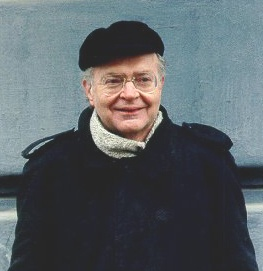
\includegraphics[width=0.4\linewidth]{images/knuth}
    \caption{Knuth}
    \label{fig:my_label}
\end{figure}